% Standalone companion note to MathematicJournal/StackingHelix.tex.
% Compile with: latexmk -pdf JointFaceRotationAddendum.tex
% No external figures, bibliography files, or journal class are needed.
\documentclass[11pt,letterpaper]{article}
\usepackage[T1]{fontenc}
\usepackage[utf8]{inputenc}
\usepackage{lmodern}
\usepackage[margin=0.9in]{geometry}
\usepackage{amsmath,amssymb,amsthm}
\usepackage{booktabs,array,tabularx}
\usepackage{microtype}
\usepackage{tikz}
\usetikzlibrary{arrows.meta}
\usepackage{fancyhdr}
\usepackage{hyperref}
\hypersetup{colorlinks=true,linkcolor=blue!45!black,citecolor=blue!45!black,
  urlcolor=blue!45!black,pdftitle={A Closed Form for the Screw Rotation of a Segmented Helix},
  pdfauthor={Robert L. Read}}
\pagestyle{fancy}
\fancyhf{}
\fancyhead[L]{\small Public Invention}
\fancyhead[R]{\small Joint-face rotation: working note}
\fancyfoot[C]{\thepage}
\setlength{\headheight}{14pt}
\setlength{\parskip}{0.35em}
\setlength{\parindent}{0pt}
\renewcommand{\arraystretch}{1.22}
\newtheorem{theorem}{Theorem}
\newcommand{\NB}{\vec N_B}
\newcommand{\NC}{\vec N_C}
\newcommand{\Rot}{\operatorname{Rot}}
\newcommand{\tr}{\operatorname{tr}}
\newcommand{\eff}{\tau_{\mathrm{eff}}}
\newcommand{\aj}{\alpha_j}
\newcommand{\gj}{\gamma_j}
\newcommand{\degc}{^{\circ}}
\newcommand{\ct}{\cos\theta}
\newcommand{\nn}{\vec n}
\newcommand{\uu}{\vec u}
\newcommand{\ee}{\vec e}

\title{A Closed Form for the Screw Rotation\\of a Segmented Helix\\[0.4em]
  \large A companion note to the Joint Face Normal Method}
\author{Robert L. Read\\Public Invention}
\date{October 1, 2026 \quad---\quad Working draft, version 0.1}

\begin{document}
\maketitle
\thispagestyle{empty}
\begin{abstract}
The Joint Face Normal Method constructs the rigid motion between successive
identical subunits of a periodic chain. Its rotational part admits a simple
closed form. If $\aj$ is the smallest rotation that opposes the two joint-face
normals and $\eff$ is the subsequent twist about the joint line, then
\[
  \boxed{\cos\frac{\theta}{2}
    =\cos\frac{\aj}{2}\left|\cos\frac{\eff}{2}\right|.}
\]
Here $\theta\in[0,\pi]$ is the principal rotation angle of the full rigid
motion. We prove the result, specify its twist convention, and give exact
expressions reproducing all 23 nonzero-radius rows in the original Platonic
helix catalog. Five straight-joint cases require distinguishing the rotation
of the subunits from the geometry of the joint points. Translation and the
remaining helix parameters are left for subsequent work.
\end{abstract}

\section{Purpose and terminology}
This note records a result for discussion with colleagues and for the
segmented-helixes repository. It supplements, rather than revises, the
2022 paper~\cite{read2022}. The relevant construction is the \emph{Joint Face
Normal Method} in Sections 2.15--2.17 of that paper. We retain its joint
points $B,C$, normalized face normals $\NB,\NC$, joint plane, joint line,
joint twist $\tau$, and screw rotation $\theta$.

Define the \emph{joint-face alignment angle}
\begin{equation}\label{eq:alpha}
  \aj=\arccos(-\NB\cdot\NC),\qquad 0\leq\aj\leq\pi.
\end{equation}
This was called $\alpha$ in the exploratory discussion; the subscript avoids
confusion with the original paper's $\alpha(\tau)$ in the Twist Spectrum proof.
For adjacent faces of a convex polyhedron, $\aj$ is its interior dihedral angle.

The essential convention is that $\eff$ is measured \emph{after the shortest
normal-aligning rotation}. When an existing out-vector or software reference
agrees with that choice, $\eff=\tau$. A reference phase may otherwise be
needed; Section~\ref{sec:phase} defines it without fitting it to a table.

\newpage
\section{The joint-face rotation theorem}\label{sec:proof}
\begin{theorem}[Joint-face rotation]
Suppose $0<\aj<\pi$. Let $A$ be the shortest rotation sending $\NB$ to
$-\NC$. After this alignment, apply a twist $\eff$ about the joint line,
using $\NC$ as its oriented axis. For the resulting rotational part
$R=\Rot(\NC,\eff)A$, its principal angle $\theta\in[0,\pi]$ satisfies
\begin{align}
  \cos\frac{\theta}{2}
    &=\cos\frac{\aj}{2}\left|\cos\frac{\eff}{2}\right|,\label{eq:half}\\
  \cos\theta
    &=\frac{(1+\cos\aj)(1+\cos\eff)}{2}-1.\label{eq:cos}
\end{align}
For $-\pi\leq\eff\leq\pi$, the absolute value in~\eqref{eq:half}
can be omitted.
\end{theorem}

\begin{proof}
The shortest alignment has angle $\aj$ and unit axis
\[
  \uu=\frac{\NB\times(-\NC)}{\sin\aj}.
\]
Thus $\uu\cdot\NC=0$: the alignment axis is perpendicular to the
joint line. Choose a right-handed orthonormal basis in which $\uu$ is
the $x$-axis and $\NC$ is the $z$-axis. This conjugates $R$ and preserves
its trace. In these coordinates,
\[
  A=\begin{pmatrix}
    1&0&0\\0&\cos\aj&-\sin\aj\\0&\sin\aj&\cos\aj
  \end{pmatrix},\qquad
  D=\begin{pmatrix}
    \cos\eff&-\sin\eff&0\\\sin\eff&\cos\eff&0\\0&0&1
  \end{pmatrix}.
\]
Multiplying $R=DA$ gives
\[
  \tr R=\cos\eff+\cos\eff\cos\aj+\cos\aj.
\]
Since a proper three-dimensional rotation obeys
$\cos\theta=(\tr R-1)/2$, this proves~\eqref{eq:cos}. Factoring gives
\[
  1+\cos\theta=\frac{(1+\cos\aj)(1+\cos\eff)}2,
  \qquad
  \cos^2\frac\theta2=\cos^2\frac\aj2\cos^2\frac\eff2.
\]
Taking the nonnegative square root proves~\eqref{eq:half}.
\end{proof}

The homogeneous rigid motion is $T=\bigl(\begin{smallmatrix}R&\vec t\\0&1\end{smallmatrix}\bigr)$.
Its translation $\vec t$ therefore cannot change $\theta$. Equivalently,
the quaternion product has scalar part
$\cos(\aj/2)\cos(\eff/2)$, because its constituent axes are perpendicular.
The absolute value handles the two quaternion representatives of the same
rotation.

Consequently $\theta(\eff)=\theta(-\eff)$,
$\theta(0)=\aj$, and $\aj\leq\theta\leq\pi$.
These statements concern rotation magnitude; they do not determine
handedness, axial travel, or whether the chain closes.

\newpage
\section{Relating the theorem to the paper's twist}\label{sec:phase}
\subsection{A reference phase for any normal-aligning baseline}
Let $R_0$ be the zero-twist rotation prescribed by an out-vector convention
or implementation. It makes the faces flush, so $R_0\NB=-\NC$.
The rotation $G=R_0A^{-1}$ fixes $\NC$. Hence it is a rotation about that
normal: $G=\Rot(\NC,\gj)$, where $\gj$ is defined modulo $2\pi$.
Applying the paper's additional twist gives
\begin{equation}\label{eq:phase}
  R=\Rot(\NC,\tau)R_0
   =\Rot(\NC,\tau+\gj)A,\qquad
  \boxed{\eff=\tau+\gj\pmod{2\pi}.}
\end{equation}
The theorem now applies. This phase depends on the chosen reference;
it is not determined by the two normals alone. For any unit vector
$\vec v\perp\NC$, it can be measured by
\[
  \gj=\operatorname{atan2}\!\left(
   \NC\cdot(\vec v\times G\vec v),\ \vec v\cdot G\vec v\right).
\]
Thus a discrepancy of twist conventions can be resolved from the baseline
rotation or the face-attached out vectors, rather than inferred from a
desired value of $\theta$.

\subsection{Why the Platonic checks use the tabulated twist directly}
The repository's \texttt{adjoinPrism} uses two shortest rotations through the
object-axis direction $\ee=(C-B)/\|C-B\|$. Write $S(\vec a,\vec b)$ for
the shortest rotation from $\vec a$ to $\vec b$. Its forward baseline is
\begin{equation}\label{eq:baseline}
  R_0=S(\ee,\NC)\,S(\NB,-\ee).
\end{equation}
For the face centers of a regular solid, with its center taken as the origin,
$B=\rho\NB$ and $C=\rho\NC$ for the same $\rho>0$. Therefore
\[
  \ee=\frac{\NC-\NB}{\sqrt{2(1-s)}},\qquad s=\NB\cdot\NC.
\]
Both rotations in~\eqref{eq:baseline} have axis parallel to
$\NB\times(-\NC)$, and
\[
  \NB\cdot(-\ee)=\ee\cdot\NC=\sqrt{\frac{1-s}{2}}
   =\cos\frac{\aj}{2}.
\]
Each has angle $\aj/2$. Their product is exactly $A$, so $\gj=0$.
This establishes the reference convention for the nonparallel Platonic
checks from geometry and the implementation, independently of their
numerical agreement.

For an arbitrary prism, the object axis need not lie in the plane of the
two normals, and this two-stage baseline may have $\gj\ne0$.
For example, with $\ee=(0,0,1)$,
$\NB=(1,0,-1)/\sqrt2$, and $\NC=(0,1,1)/\sqrt2$, the alignment angle is
$60\degc$, but~\eqref{eq:baseline} has principal angle
$62.7994\degc$ at $\tau=0$. Its phase is
$\gj=\arccos(2\sqrt2/3)=19.4712\degc$.
The effective-twist formula gives the correct value.

\newpage
\section{Face classes without arbitrary face numbers}\label{sec:classes}
Fix the Base Joint Face $B$ and classify distinct Chained Joint Faces $C$
by the invariant $\NB\cdot\NC$. The classes below replace the software's
arbitrary C-face numbering. $A$ denotes adjacent, $S,T,F$ successive
normal-dot-product classes, and $O$ opposite. Multiplicities count faces,
not the catalog's shape analogs.

\begin{center}\small
\begin{tabular}{llrc}
\toprule
Solid & Class & Number of faces & $\cos\aj=-\NB\cdot\NC$\\
\midrule
Tetrahedron & $A$ & 3 & $1/3$\\
Cube & $A$ & 4 & $0$\\
     & $O$ & 1 & $1$\\
Octahedron & $A$ & 3 & $-1/3$\\
           & $S$ & 3 & $1/3$\\
           & $O$ & 1 & $1$\\
Dodecahedron & $A$ & 5 & $-1/\sqrt5$\\
             & $S$ & 5 & $1/\sqrt5$\\
             & $O$ & 1 & $1$\\
Icosahedron & $A$ & 3 & $-\sqrt5/3$\\
            & $S$ & 6 & $-1/3$\\
            & $T$ & 6 & $1/3$\\
            & $F$ & 3 & $\sqrt5/3$\\
            & $O$ & 1 & $1$\\
\bottomrule
\end{tabular}
\end{center}

\subsection{The dodecahedron from its dual}
Put $\varphi=(1+\sqrt5)/2$. Dodecahedral face normals point toward the
vertices of an icosahedron. Use the twelve vectors
\[
 (0,\pm1,\pm\varphi),\quad
 (\pm1,\pm\varphi,0),\quad
 (\pm\varphi,0,\pm1),
\]
all divided by $\sqrt{1+\varphi^2}$, and fix
$\NB=(0,1,\varphi)/\sqrt{1+\varphi^2}$. Their dot products with
$\NB$, excluding $B$ itself, are
$1/\sqrt5,-1/\sqrt5,-1$ with counts $5,5,1$. For example,
$(1,\varphi,0)$ yields
$\varphi/(1+\varphi^2)=1/\sqrt5$.

\subsection{The icosahedron from its dual}
Icosahedral normals point toward the twenty vertices of a dodecahedron.
Take $(\pm1,\pm1,\pm1)$ and
\[
 (0,\pm\varphi^{-1},\pm\varphi),\quad
 (\pm\varphi^{-1},\pm\varphi,0),\quad
 (\pm\varphi,0,\pm\varphi^{-1}),
\]
all divided by $\sqrt3$. With $\NB=(1,1,1)/\sqrt3$,
the other nineteen dot products are
\[
 \sqrt5/3,\quad 1/3,\quad -1/3,\quad -\sqrt5/3,\quad -1,
\]
with counts $3,6,6,3,1$.
These facts follow directly from $\varphi+\varphi^{-1}=\sqrt5$ and
$\varphi-\varphi^{-1}=1$.

\newpage
\section{Exact catalog checks}\label{sec:catalog}
All twists and catalog values below are from Table 1 of the original
paper and the supplied LaTeX source~\cite{read2022,repository}.
The convention established in Section~\ref{sec:phase} gives $\eff=\tau$.
Every entry means $\theta=\arccos(\text{listed exact expression})$;
angles in the last two columns are in degrees. Numerical agreement is
checked at the catalog's three-decimal precision. The proof, rather than
agreement alone, establishes the identity.

\subsection{Tetrahedral, cubic, and octahedral cases}
\begin{center}\small
\setlength{\tabcolsep}{5pt}
\begin{tabular}{llrcrr}
\toprule
Name & Class & $\tau$ & Exact $\cos\theta$ & Computed & Catalog\\
\midrule
Tetratorus & Tet $A$ & $0$ & $1/3$ & $70.5288$ & $70.529$\\
Tetrahelix & Tet $A$ & $-120$ & $-2/3$ & $131.8103$ & $131.810$\\
\addlinespace
Cubatorus & Cub $A$ & $0$ & $0$ & $90.0000$ & $90.000$\\
Blockhelix & Cub $A$ & $-90$ & $-1/2$ & $120.0000$ & $120.000$\\
\addlinespace
Octagear & Oct $A$ & $0$ & $-1/3$ & $109.4712$ & $109.471$\\
Octaspiky & Oct $A$ & $-120$ & $-5/6$ & $146.4427$ & $146.443$\\
Treestar & Oct $S$ & $0$ & $1/3$ & $70.5288$ & $70.529$\\
Octamedium & Oct $S$ & $-120$ & $-2/3$ & $131.8103$ & $131.810$\\
\bottomrule
\end{tabular}
\end{center}
The octahedral names follow the supplied manuscript. The face classes
and exact values remain unambiguous if labels differ elsewhere.

\subsection{Dodecahedral cases}
\begin{center}\small
\setlength{\tabcolsep}{5pt}
\begin{tabular}{llrcrr}
\toprule
Name & Class & $\tau$ & Exact $\cos\theta$ & Computed & Catalog\\
\midrule
Dodecagear & $A$ & $0$ & $-1/\sqrt5$ & $116.5651$ & $116.565$\\
Dodecashaft & $A$ & $-72$ & $(\sqrt5-15)/20$ & $129.6575$ & $129.657$\\
Dodecadoubler & $A$ & $-144$ & $-1/2-1/\sqrt5$ & $161.3006$ & $161.301$\\
Dodecadonut & $S$ & $0$ & $1/\sqrt5$ & $63.4349$ & $63.435$\\
Dodecacorkscrew & $S$ & $-72$ & $-1/2+1/\sqrt5$ & $93.0258$ & $93.026$\\
The Alternater & $S$ & $-144$ & $-3/4-\sqrt5/20$ & $149.5197$ & $149.520$\\
\bottomrule
\end{tabular}
\end{center}

For example, Dodecacorkscrew has $\cos\aj=1/\sqrt5$ and
$\cos\tau=\cos72\degc=(\sqrt5-1)/4$. Therefore
\[
  \cos\theta
  =\frac{(1+1/\sqrt5)(1+(\sqrt5-1)/4)}{2}-1
  =-\frac12+\frac1{\sqrt5}.
\]
Thus $\theta=\arccos(-1/2+1/\sqrt5)=93.0258445\degc$.
There are six nonzero-radius dodecahedral checks; Dodecabeam is discussed
in Section~\ref{sec:degenerate}.

\newpage
\subsection{Icosahedral cases}
\begin{center}\small
\setlength{\tabcolsep}{6pt}
\begin{tabular}{llrcrr}
\toprule
Name & Class & $\tau$ & Exact $\cos\theta$ & Computed & Catalog\\
\midrule
Icosa Tree Star & $A$ & $0$ & $-\sqrt5/3$ & $138.1897$ & $138.190$\\
Two Strands & $A$ & $120$ & $-(9+\sqrt5)/12$ & $159.4456$ & $159.446$\\
Planar point cluster & $S$ & $0$ & $-1/3$ & $109.4712$ & $109.471$\\
Rock Candy & $S$ & $120$ & $-5/6$ & $146.4427$ & $146.443$\\
Big Icosacorkscrew & $T$ & $45$ & $(\sqrt2-1)/3$ & $82.0638$ & $82.064$\\
Icosacorkscrew & $T$ & $-75$ & $(\sqrt6-\sqrt2-2)/6$ & $99.2526$ & $99.253$\\
Quasi-planar & $T$ & $165$ & $-(2+\sqrt6+\sqrt2)/6$ & $167.7643$ & $167.764$\\
The Wheel & $F$ & $0$ & $\sqrt5/3$ & $41.8103$ & $41.810$\\
Slow Twist & $F$ & $120$ & $(\sqrt5-9)/12$ & $124.3094$ & $124.309$\\
\bottomrule
\end{tabular}
\end{center}

The three class-$T$ twists $45\degc,-75\degc,165\degc$ are separated
by $120\degc$, as triangular vertex matching requires. They test the same
face geometry with three distinct orientations. For Icosacorkscrew,
\[
  \cos\theta
  =\frac{(1+1/3)(1+\cos75\degc)}{2}-1
  =\frac{\sqrt6-\sqrt2-2}{6},
\]
using $\cos75\degc=(\sqrt6-\sqrt2)/4$.

\subsection{What is being verified}
Together, these tables give $2+2+4+6+9=23$ checks with nonzero joint-helix
radius. For such a joint orbit, the angular advance of consecutive joints
is the principal rotation angle of $R$. No reference phase was chosen to
force these matches: the normals supply $\aj$, the original catalog
supplies $\tau$, and the face-center argument supplies $\gj=0$.

\begin{center}
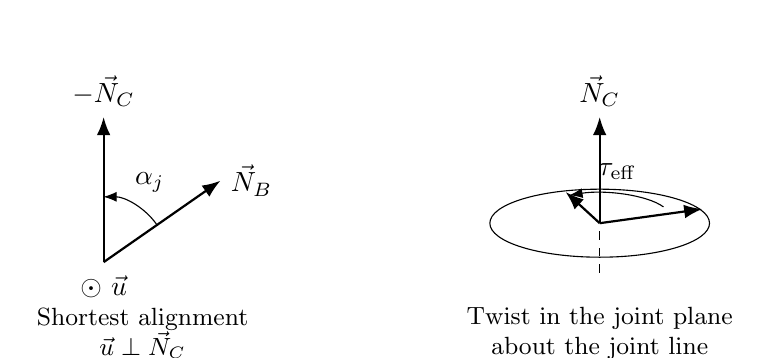
\begin{tikzpicture}[>=Latex,scale=0.9]
  \begin{scope}
    \draw[->,thick] (0,0)--(0,2.05) node[above] {$-\NC$};
    \draw[->,thick] (0,0)--(1.65,1.15) node[right] {$\NB$};
    \draw[->] (0.75,0.53) arc[start angle=35,end angle=90,radius=0.92];
    \node at (0.65,1.12) {$\aj$};
    \node at (0,-0.35) {$\odot\ \uu$};
    \node[align=center,font=\small] at (0.55,-1.0) {Shortest alignment\\$\uu\perp\NC$};
  \end{scope}
  \begin{scope}[shift={(7,0)}]
    \draw (0,0.55) ellipse (1.55 and 0.48);
    \draw[dashed] (0,-0.15)--(0,0.55);
    \draw[->,thick] (0,0.55)--(0,2.05) node[above] {$\NC$};
    \draw[->,thick] (0,0.55)--(1.45,0.75);
    \draw[->,thick] (0,0.55)--(-0.48,0.99);
    \draw[->] (0.9,0.78) arc[start angle=25,end angle=115,x radius=1.0,y radius=0.34];
    \node at (0.25,1.28) {$\eff$};
    \node[align=center,font=\small] at (0,-1.0) {Twist in the joint plane\\about the joint line};
  \end{scope}
\end{tikzpicture}
\end{center}
\small The diagram is schematic. The theorem uses only the perpendicularity
of the two rotation axes, not any particular polyhedron.\normalsize

\newpage
\section{Parallel normals and straight-joint degeneracies}\label{sec:degenerate}
\subsection{What the normals do and do not determine}
If $\NB=-\NC$, then $\aj=0$ and the shortest alignment is the identity.
The normals impose no condition on a spin about their common line. Once
the out-vector reference fixes that spin,
\[
  \theta=\arccos(\cos\eff)=|\eff|
    \quad\text{for }-\pi\leq\eff\leq\pi.
\]
There is no failure of the formula at $\aj=0$. If instead $\NB=\NC$,
then $\aj=\pi$: choose any perpendicular half-turn axis. Every resulting
face-opposing rotation has principal angle $\pi$, as the formula predicts.
The normals alone do not select the entire transformation in either case.

\subsection{A straight joint line hides subunit rotation}
Let a screw motion rotate by any angle about an axis and translate along
that axis. A point \emph{on} the axis advances in a straight line, independently
of the rotation. Thus $r=0$ makes $\theta$ unidentifiable from the joint points.
The original paper explicitly recognizes this in its straight-line special
case: the point method leaves $\theta$ undefined, while orientation data can
supply it. A listed value of zero for the straight-joint curve does not prove
that the full rigid motion has $R=I$.

For the repository's face-center baseline, the full principal rotations
are as follows. These are predictions of the actual rotation construction;
they are not replacements for the catalog's convention for a degenerate
joint curve.
\begin{center}\small
\begin{tabular}{llrrrr}
\toprule
Name & Face class & $\aj$ & $\tau$ & Full $R$: $\theta$ & Catalog $\theta$\\
\midrule
Boxbeam & Cub $O$ & $0$ & $-180$ & $180$ & $0$\\
Staircase & Cub $A$ & $90$ & $-180$ & $180$ & $0$\\
Octabeam & Oct $O$ & $0$ & $-60$ & $60$ & $0$\\
Dodecabeam & Dod $O$ & $0$ & $-108$ & $108$ & $0$\\
Pearlshaft & Ico $O$ & $0$ & $-60$ & $60$ & $0$\\
\bottomrule
\end{tabular}
\end{center}
All five have $r=0$ in the catalog. The Staircase also shows that a
straight-joint degeneracy can occur with nonparallel normals. Rotations of
an unmarked solid may additionally be equivalent under its own symmetries;
here $R$ refers to the specified motion of a labeled subunit.

This corrects an interpretation in the exploratory discussion: the
Dodecabeam and Pearlshaft rows do \emph{not} establish cancelling phases
of $108\degc$ and $60\degc$. Their joint-point data cannot establish a
phase at all. In the code baseline for these centered opposite faces,
$R_0=I$ and $\gj=0$; the imposed twist remains in $R$.

\newpage
\section{Scope, reproducibility, and subsequent work}
The compact formula is
\[
  \boxed{\theta=2\arccos\!\left(
    \cos\frac{\aj}{2}\left|\cos\frac{\eff}{2}\right|\right),
    \qquad \aj=\arccos(-\NB\cdot\NC).}
\]
Its origin is the classical composition of rotations about perpendicular
axes. The contribution of this note is the application to the Joint Face
Normal Method, an explicit account of its twist reference, and exact
catalog expressions. No claim of priority for the rotation identity or of
an exhaustive literature review is made. Related tetrahelix work is already
discussed in the original paper~\cite{sadler2019}.

For fixed $\eff$, neither the object length nor the translation vector enters
$\theta$. If a numerical twist reference is tied to joint positions, those
positions can affect $\gj$ and must be included when translating that
reference to $\eff$. Consequently a bare pair $(\aj,\tau)$ is sufficient
only when the zero-twist convention has been specified.

The formula does not determine the screw axis, radius $r$, axial advance
$d$, or helix angle $\phi$. For those, the next step is to combine the
rotation with $\vec t$, compute the screw axis, and locate a chosen joint
relative to it. Nor does the formula ensure a physically nonintersecting
stack or a closed torus. At $R=I$, the separate pure-translation or identity
cases will also need to be retained.

\subsection*{Reproducible checks}
The companion script \texttt{verify\_joint\_face\_rotation.py} uses only
Python's standard library. It checks the 23 exact expressions against the
catalog's rounded values, enumerates the face-normal classes, compares
matrix products with the half-angle law, and tests both the general
reference phase and the five straight-joint cases. In the latter it verifies
the full rotation and the collinearity of successive joints separately.

The source baseline is repository revision
\texttt{8be3839de2204b966c8aedb7c28f6a6f5c18076e}, specifically
\texttt{MathematicJournal/StackingHelix.tex} and
\texttt{js/segment\_helix\_math.js}, including \texttt{adjoinPrism} and
\texttt{PointAxis}. The original manuscript and implementation are not
changed by this companion note. The standalone source compiles using
ordinary pdfLaTeX and needs no external images or bibliography file.

\textbf{Preparation.} Developed through discussion between Robert L. Read
and ChatGPT (OpenAI), with assistance in derivation, source inspection,
verification, and drafting. This is a working note for colleague review.

\begin{thebibliography}{9}
\small
\setlength{\itemsep}{0.15em}
\bibitem{read2022}
R. L. Read, \emph{Calculating the Segmented Helix Formed by Repetitions of
Identical Subunits thereby Generating a Zoo of Platonic Helices},
Mathematics \textbf{10}(14), 2533 (2022).
\href{https://doi.org/10.3390/math10142533}{doi:10.3390/math10142533}.

\bibitem{repository}
Public Invention, \emph{segmented-helixes} source repository.
\href{https://github.com/PubInv/segmented-helixes}{GitHub repository}.
Revision and source paths are specified above.

\bibitem{sadler2019}
G. Sadler, F. Fang, R. Clawson, and K. Irwin,
\emph{Periodic Modification of the Boerdijk--Coxeter Helix (Tetrahelix)},
Mathematics \textbf{7}(10), 1001 (2019).
\href{https://doi.org/10.3390/math7101001}{doi:10.3390/math7101001}.
\end{thebibliography}
\end{document}
